We are now almost in position to use the formula of Proposition \ref{prop:formula_char}: the character tables of the groups are supposed to be given, as we dispose of efficient group algorithms in the literature to compute them, from Algorithm \ref{algo:l_class} we now know how the efficiently compute the bicharacter of $\kbf \lc(e)$ as a $\kbf M \otimes \kbf G_e^{op}$-module for some idempotent $e \in M$. It remains to compute the bicharacter of $N_e(\kbf \lc(e))$ as a $\kbf M \otimes \kbf G_e^{op}$-module, which we discuss now.

Let $L = \lc(e)$. Recall that, by definition, $N_e(\kbf L) = \{x \in \kbf L \sepp  eMx = 0\}$.
Taking $L$ as a basis for $\kbf L$, we can form a matrix with rows indexed by $M \times L$ and columns indexed by $L$, with the coefficient at $((m, l), l') = 1$ if $eml = l'$ and 0 otherwise. Computing the kernel of this matrix yields a basis for $N_e(\kbf L)$ but is extremely inefficient as the number of rows is many times the cardinality of the monoïd.

Notice first that for any $m \in M$, $em \leqr e$ so we can consider only the elements of $M$ that are $\rc$-smaller than $e$. 
Conversely, recall that the structure of $\kbf M$-module on $M$ is defined by $m\cdot l = ml$ if $ml \in L$ and $0$ otherwise and that this latter case happens if $ml  \leql l$. Since if $m \leql l$ implies $ml \leql l$ we have that the $(m, l)$-th row of the matrix is null and that we may omit it. This shows that we need only to consider the element of $M$ that are not $\lc$-below $e$. Together with the previous point, this means that the similarly defined matrix but whose rows are only indexed by $\rc(e) \times L$ has the same kernel. This is good news, as we may now exploit the structure of the $\jc$-class given by Green's Lemma to further reduce the dimension of this matrix. Indeed, another consequence of Green's Lemma is the so called "Location Theorem" from Clifford and Miller. A proof can be found in \cite[Theorem 1.11]{Pin:Automata}

\begin{lemme}[Location Theorem]
	Let $r, l$ be two elements in the same $\jc$-class.
	We have:
	\[rl = \left\{\begin{aligned}
	& \gamma \in \rc(r) \cap \lc(l) \textrm{ if } \lc(r)\cap\rc(l) \textrm{ contains an idempotent},\\
	& \gamma <_{\jc} l, r \textrm{ otherwise}.
	\end{aligned}\right.\]
\end{lemme}

\begin{figure}[h!]\label{fig:location}
	\centering
	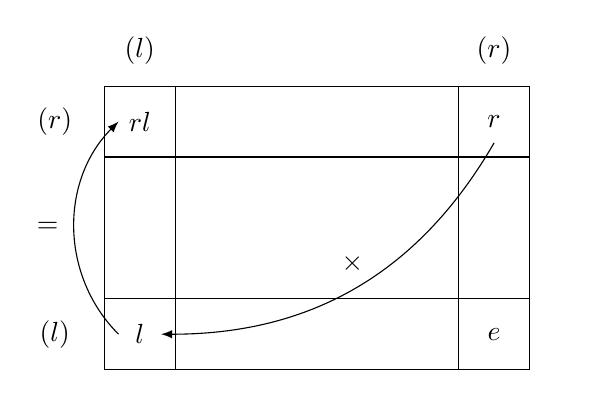
\begin{tikzpicture}[scale = 0.9]
	\tikzstyle{fleche}=[->,>=latex,rounded corners=4pt]
	\node at (0,0){$l$};
	\node at (0,3){$rl$};
	\node at (5,0){$e$};
	\node at (5,3){$r$};
	\draw (-.5,3.5) -- (-.5, -.5);
	\draw (.5,3.5) -- (.5, -.5);
	\draw (5.5,3.5) -- (5.5, -.5);
	\draw (4.5,3.5) -- (4.5, -.5);
	\draw (-.5,3.5) -- (5.5, 3.5);
	\draw (-.5,2.5) -- (5.5, 2.5);
	\draw (-.5,.5) -- (5.5, .5);
	\draw (-.5,-.5) -- (5.5, -.5);
	
	\draw[->, >=latex, bend left = 45] (-.3, 0) to (-.3, 3);
	\node at (-1.3, 1.5){$=$};
	\draw[->, >=latex, bend left] (5,2.7) to (0.3,0);
	\node at (3, 1){$\times$};
	
	\node at (-1.2, 3){$\rc(r)$};
	\node at (-1.2, 0){$\rc(l)$};
	\node at (0, 4){$\lc(l)$};
	\node at (5, 4){$\lc(r)$};
	\node at (6, 0){};
	
	\end{tikzpicture}
	\caption{Location Theorem\\ {\small Since there is an idempotent $e$ in $\lc(r)\cap \rc(l)$, $rl$ stays in the same $\jc$-class, in $\lc(l) \cap \rc(r)$.}}
\end{figure}

\begin{lemme}
	Let $e \in M$ be an idempotent, $R = \rc(e)$ its $\rc$-class and $R'$ another $\rc$-class of $\jc(e)$. Let $(\lambda, \lambda')$ be a left Green pair for $(L, L')$. Then $(\lambda e, e\lambda')$ is a left Green pair for $(R, R')$.
	
	Similarly, if $L = \lc(e)$, $L'$ is a $\lc$-class of $\jc(e)$ and $(\rho, \rho')$ is a right Green pair for $(L, L')$, then $(e\rho, \rho'e)$ is a right Green pair for $(L, L')$
\end{lemme}

\begin{proof}
	Let $g$ be any element of $\hc(e)$ and $g' = \lambda g$. Since $e$ is idempotent, $\hc(e)$ is a group with identity $e$ so we have $e\lambda'\lambda e g = e \lambda'\lambda g = eg = g$ and $\lambda ee\lambda' g' = \lambda eg = \lambda g = g'$ which, from Green's Lemma, make $(\lambda e, e\lambda')$ a left Green pair for $(L, L')$. A similar argument applies for the second part of the proposition.
\end{proof}

\begin{rmk}
	This lemma means that for a regular $\jc$-class $J$ and for any two $\lc$-class (or $\rc$-class) it contains, we may choose a corresponding Green pair among the elements of those two classes.
\end{rmk}

\begin{prop}\label{prop:equations}
	Let $e \in M$ be an idempotent and $H = \hc(e), L = \lc(e), R = \rc(e)$ and $J = \jc(e)$. 
	For each $\rc$-class $R' \subset J$, we choose a left Green pair $(l, l') \in J^2$. We denote by $\mathfrak{L}$ the set of all $l$ for the chosen left Green pairs. We define $\mathfrak{R}$ similarly.
	Then $N_e$ is the set of solutions of :
	\[\forall r \in \mathfrak{R}, \forall g \in H,\quad \sum_{l \in \mathfrak{L}} \ind_H(rl)x_{l(rl)\inv g} = 0\]
\end{prop}

\begin{proof}
	Consider an element $a \in R$. $a$ can be written in a unique way as $gr$, with $g \in G$ and $r \in \mathfrak{R}$ corresponding to $\lc(a)$. Similarly, an element $b$ in $L$ as a unique decomposition as $l\gamma, l \in \mathfrak{L}, \gamma \in H$.
	For an element $x \in \kbf L$ we note:
	\[x = \sum_{l \in \mathfrak{L}, \gamma \in H}x_{l\gamma}l\gamma\]
	its decomposition over the basis $L$.
	
	We want to find the equations that describe $\ker(gr\mul{L})$ (where $gr\mul{L}$ is the linear map on $\kbf L$ obtained by extending the monoid's multiplication by linearity). From the Location Theorem, we get that $\im(gr\mul{L}) \subset \kbf H$.
	For $k \in H$, denote by $f_{k, gr}$ the $k$-th coordinate function of $gr\mul{L}$.
	Because $gr\mul{L}$ acts combinatorially on $\kbf L$, we have :
	\[f_{k, gr}(x) = \sum_{l \in \mathfrak{L}, \gamma \in H} \ind_{\{k\}}(grl\gamma)x_{l \gamma}\]
	
	Note that $x_{l \gamma}$ appears in the sum if and only if $grl\gamma = k$. From the Location Theorem, and because we choose $l \in L, r \in R$, we have $grl\gamma = k \textrm{ if and only if } rl \in H \textrm{ and } \gamma = (rl)\inv g\inv k$
	and thus the equation becomes:
	\[f_{k, gr}(x) = \sum_{l \in \mathfrak{L}} \ind_H(rl)x_{l(rl)\inv g\inv k}.\]
	For $x$ to be in $\ker(gr\mul{L})$, $x$ must cancel simultaneously $f_{k, gr}$ for all $k\in H$. We now have a set of equations for $ker(gr\mul{L})$, and we can deduce that the set of equations
	\[\forall r \in \mathfrak{R}, \forall g,k \in H, \quad f_{k, gr}(x) = \sum_{l \in \mathfrak{L}, \gamma \in H} \ind_H(rl)x_{l (rl)\inv g\inv k} = 0\]
	describes $N_e(\kbf L)$.
	However, the equation system is redundant as the equation $f_{k, gr}(x) = 0$ is the same for all pairs $(g, gk')$ with $k' \in H$. Removing the duplicates equation gives the system announced in the proposition.
\end{proof}

\begin{lined}
	\begin{ex}[$N_e$ in the case of an aperiodic monoid]
		As in Example \ref{ex:aperiodic_bichar}, let us consider the case of a $\jc$-class with trivial $\hc$-classes. In this case, we have $L = \mathfrak{L}, R = \mathfrak{R}$ and $H = \{1_H\}$, so the equations become:
		\[\forall r \in R, \quad \sum_{l\in M}\ind_H(rl)x_l.\]
		Again from the Location Theorem, we have that $\ind_H(rl) = 1$ if and only if there is an idempotent in $\lc(r)\cap\rc(l)$. So if we form a matrix $A$ with rows indexed by $L$ and columns indexed by $R$, and with coefficients 1 at $(\lc(r),\rc(l))$ if $\lc(r)\cap \rc(l)$ contains an idempotent and 0 otherwise, the above equations becomes :
		\[(x_l)_{l\in L}^T A = 0,\]
		that is, in the case of an $\hc$-trivial $\jc$-class, $N_e(\kbf L)$ is the left kernel of the eggbox picture seen as a $\{0, 1\}$-matrix. 
	\end{ex}
\end{lined}

Note that given this set of equations, we can compute the character $\chi_{\kbf M \otimes \kbf G_e^{op}}^{N_e(\kbf\lc(e))}$ from the formula in Proposition \ref{prop:formula_char} using classical linear algebra algorithms to find a basis of $N_e(\kbf\lc(e))$ and then computing the value of the character at any $(m, g) \in C_M \times C_{G_e}$ by iterating over the basis vectors, applying $(m, g)$ as a linear map and computing the relevant coefficient in the image vector.
